\documentclass[border=0pt]{standalone}
\usepackage{pgfplots}
%\pgfplotsset{width=7cm,compat=1.8}
\usepackage{pgfplotstable}
\renewcommand*{\familydefault}{\sfdefault}
\usepackage{sfmath}
%\pgfplotsset{width=7cm,compat=1.8}
%\usetikzlibrary{positioning, arrows, shapes, shadows, calc, fit}
%\usepackage{pgfplots}
%\usepackage{subcaption}


\begin{document}
	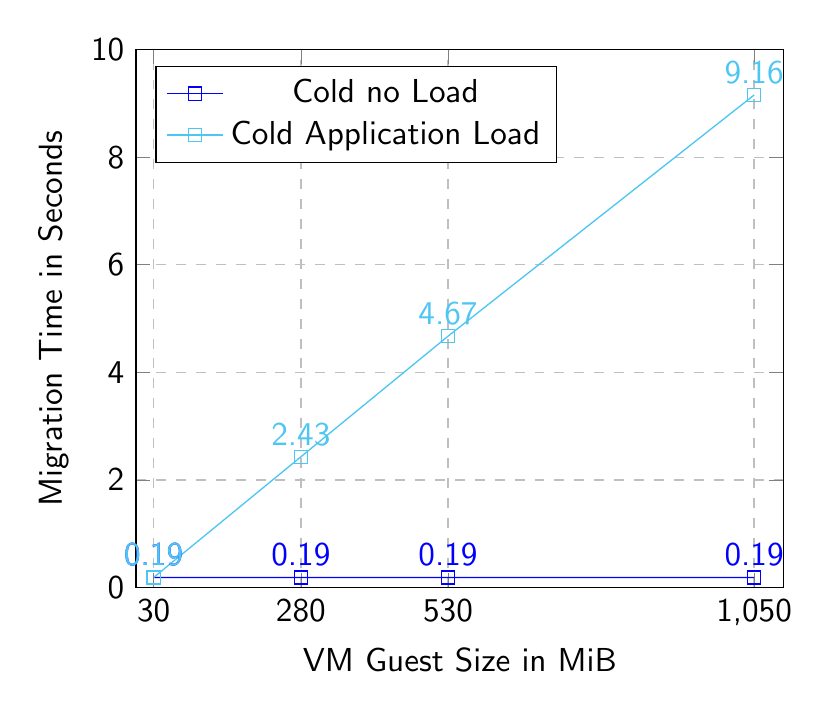
\begin{tikzpicture}[scale=1.2]
	\begin{axis}[
	%title={Temperature dependence of CuSO$_4\cdot$5H$_2$O solubility},
	nodes near coords,
	xlabel={VM Guest Size in MiB},
	ylabel={Migration Time in Seconds},
	xmin=0, xmax=1100,
	ymin=0, ymax=10,
	xtick={30,280,530,1050},
	ytick={0,2,4,6,8,10},
	legend pos=north west,
	ymajorgrids=true,
	xmajorgrids=true,
	grid style=dashed,
	]
	
	\addplot[
	color=blue,
	mark=square,
	]
	coordinates {
		(30,0.1882)(280,0.1879)(530,0.1876)(1050,0.1883)
	};
	\addplot[
	color=cyan!70,
	mark=square,
	]
	coordinates {
		(30,0.1882)(280,2.4306)(530,4.6733)(1050,9.1564)
	};
	\legend{Cold no Load, Cold Application Load}
	
	\end{axis}
	\end{tikzpicture}
\end{document}